%%%%%%%% ICML 2026 EXAMPLE LATEX SUBMISSION FILE %%%%%%%%%%%%%%%%%

\documentclass{article}

% Recommended, but optional, packages for figures and better typesetting:
\usepackage{microtype}
\usepackage{graphicx}
\usepackage{subcaption}
\usepackage{booktabs} % for professional tables

% hyperref makes hyperlinks in the resulting PDF.
% If your build breaks (sometimes temporarily if a hyperlink spans a page)
% please comment out the following usepackage line and replace
% \usepackage{icml2026} with \usepackage[nohyperref]{icml2026} above.
\usepackage{hyperref}


% Attempt to make hyperref and algorithmic work together better:
\newcommand{\theHalgorithm}{\arabic{algorithm}}

% Use the following line for the initial blind version submitted for review:
\usepackage{icml2026}

% For preprint, use
% \usepackage[preprint]{icml2026}

% If accepted, instead use the following line for the camera-ready submission:
% \usepackage[accepted]{icml2026}

\usepackage{amsmath}
\usepackage{amssymb}
\usepackage{mathtools}
\usepackage{amsthm}
\usepackage{multirow} 
\usepackage{dcolumn}  
\usepackage{booktabs} 
\usepackage{graphicx}    
% \usepackage{float} 
\usepackage{subcaption}
\newcolumntype{d}{D{.}{.}{2}} 


% if you use cleveref..
\usepackage[capitalize,noabbrev]{cleveref}

%%%%%%%%%%%%%%%%%%%%%%%%%%%%%%%%
% THEOREMS
%%%%%%%%%%%%%%%%%%%%%%%%%%%%%%%%
\theoremstyle{plain}
\newtheorem{theorem}{Theorem}[section]
\newtheorem{proposition}[theorem]{Proposition}
\newtheorem{lemma}[theorem]{Lemma}
\newtheorem{corollary}[theorem]{Corollary}
\theoremstyle{definition}
\newtheorem{definition}[theorem]{Definition}
\newtheorem{assumption}[theorem]{Assumption}
\theoremstyle{remark}
\newtheorem{remark}[theorem]{Remark}

% Todonotes is useful during development; simply uncomment the next line
%    and comment out the line below the next line to turn off comments
%\usepackage[disable,textsize=tiny]{todonotes}
\usepackage[textsize=tiny]{todonotes}

% The \icmltitle you define below is probably too long as a header.
% Therefore, a short form for the running title is supplied here:
\icmltitlerunning{Submission and Formatting Instructions for ICML 2026}

\begin{document}
\twocolumn[
  \icmltitle{TORQ: Two-Level Orthogonal Rotation for MXFP4 Quantization}

  % It is OKAY to include author information, even for blind submissions: the
  % style file will automatically remove it for you unless you've provided
  % the [accepted] option to the icml2026 package.

  % List of affiliations: The first argument should be a (short) identifier you
  % will use later to specify author affiliations Academic affiliations
  % should list Department, University, City, Region, Country Industry
  % affiliations should list Company, City, Region, Country

  % You can specify symbols, otherwise they are numbered in order. Ideally, you
  % should not use this facility. Affiliations will be numbered in order of
  % appearance and this is the preferred way.
  \icmlsetsymbol{equal}{*}

  \begin{icmlauthorlist}
    \icmlauthor{Firstname1 Lastname1}{equal,yyy}
    \icmlauthor{Firstname2 Lastname2}{equal,yyy,comp}
    \icmlauthor{Firstname3 Lastname3}{comp}
    \icmlauthor{Firstname4 Lastname4}{sch}
    \icmlauthor{Firstname5 Lastname5}{yyy}
    \icmlauthor{Firstname6 Lastname6}{sch,yyy,comp}
    \icmlauthor{Firstname7 Lastname7}{comp}
    %\icmlauthor{}{sch}
    \icmlauthor{Firstname8 Lastname8}{sch}
    \icmlauthor{Firstname8 Lastname8}{yyy,comp}
    %\icmlauthor{}{sch}
    %\icmlauthor{}{sch}
  \end{icmlauthorlist}

  \icmlaffiliation{yyy}{Department of XXX, University of YYY, Location, Country}
  \icmlaffiliation{comp}{Company Name, Location, Country}
  \icmlaffiliation{sch}{School of ZZZ, Institute of WWW, Location, Country}

  \icmlcorrespondingauthor{Firstname1 Lastname1}{first1.last1@xxx.edu}
  \icmlcorrespondingauthor{Firstname2 Lastname2}{first2.last2@www.uk}

  % You may provide any keywords that you find helpful for describing your
  % paper; these are used to populate the "keywords" metadata in the PDF but
  % will not be shown in the document
  \icmlkeywords{Machine Learning, ICML}

  \vskip 0.3in
]

% this must go after the closing bracket ] following \twocolumn[ ...

% This command actually creates the footnote in the first column listing the
% affiliations and the copyright notice. The command takes one argument, which
% is text to display at the start of the footnote. The \icmlEqualContribution
% command is standard text for equal contribution. Remove it (just {}) if you
% do not need this facility.

% Use ONE of the following lines. DO NOT remove the command.
% If you have no special notice, KEEP empty braces:
\printAffiliationsAndNotice{}  % no special notice (required even if empty)
% Or, if applicable, use the standard equal contribution text:
% \printAffiliationsAndNotice{\icmlEqualContribution}

%正文8页
%图的标题在下面
%表的标题在上方


\begin{abstract}
%随着大规模语言模型（LLMs）向实际部署迈进，微缩放格式 MXFP4（Microscaling FP4）凭借其兼顾高动态范围与硬件效率的特性，被视为下一代低比特推理的基石。然而，直接将 MXFP4 应用于 LLM 激活量化会导致显著的精度衰退。本文从理论层面剖析了 MXFP4 激活量化的误差结构，揭示了导致精度下降的根本原因在于激活分布与 MXFP4 块浮点结构之间存在的两种失衡：1.跨块方差极度不均衡：在按固定组大小进行 microscaling 时，组间方差高度不均衡, 少数高方差组主导总体量化误差并迫使共享尺度抬升，导致组内大量中小幅值激活被过度粗化。2.块内码本利用不均衡：真实激活的重尾分布与  MXFP4 几何级数码本严重失配，导致有效码字利用率极低，大量码字表示能力被闲置。
%为解决上述问题，我们提出了 TORQ (Two-level Orthogonal Rotation for MXFP4 Quantization) 。这是一种无需重训练的 PTQ 框架，旨在通过构建最优坐标变换来重塑激活空间的几何特性。 在宏观层面，TORQ 基于 Schur-Horn 定理，通过块间正交旋转实现方差的全局均衡，并从理论上证明了在凸误差假设下，该均衡配置等价于全局最小均方误差（MSE）。 在微观层面，TORQ引入最大熵原理，在组内执行正交旋转，最大化码字信息熵，使量化后激活的分布更适应fp数据分布，从而提升 MXFP4 码本的有效利用率。 在 LLaMA3和 Qwen3 等多种主流 LLM 上的实验表明，TORQ 相比现有 SOTA 方法显著提升了激活 MXFP4 PTQ 的精度：在Qwen3-32B模型上，在 WikiText 上将困惑度降至 8.43（BF16是7.61），在平均准确率上从 直接RTN的38.40% 提升至 73.63%(BF16是74.82)，成功弥合了 4-bit 浮点量化与全精度推理的鸿沟。

As Large Language Models (LLMs) advance toward practical deployment, the Microscaling FP4 (MXFP4) format has emerged as a cornerstone for next-generation low-bit inference, owing to its ability to balance high dynamic range with hardware efficiency. However, directly applying MXFP4 to LLM activation quantization inevitably leads to significant accuracy degradation. In this paper, we theoretically analyze the error structure of MXFP4 activation quantization, revealing that the root cause of this performance drop lies in two structural imbalances between activation distributions and the MXFP4 block floating-point format: (1).Extreme Inter-block Variance Imbalance: Under fixed-block microscaling, inter-block variance is highly uneven. Specifically, a minority of high-variance blocks dominate the total quantization error and force the shared scaling factor upward, resulting in the excessive coarsening of numerous small-magnitude activations within the block. 
(2).Intra-block Codebook Utilization Imbalance: The heavy-tailed distribution of real-world activations severely mismatches the MXFP4 geometric progression codebook, leading to extremely low effective codeword utilization and leaving significant representation capacity idle.
To address these challenges, we propose TORQ (Two-level Orthogonal Rotation for MXFP4 Quantization), a training-free Post-Training Quantization (PTQ) framework designed to reshape the geometric properties of the activation space through optimal coordinate transformations. 
% At the macroscopic level, TORQ leverages the Schur-Horn theorem to achieve global variance equalization via inter-block orthogonal rotation; we theoretically prove that this equilibrium configuration is equivalent to the global minimum Mean Squared Error (MSE) under convex error assumptions. 
At the macroscopic level, TORQ leverages the Schur-Horn theorem to redistribute activation energy via inter-block orthogonal rotation. Mathematically formalized as variance equalization, this process acts as a soft outlier suppression mechanism—preventing high-variance blocks from driving up the shared scaling factors and thereby preserving the precision of small-magnitude elements.
% At the microscopic level, TORQ introduces the principle of maximum entropy to execute intra-block orthogonal rotation. This maximizes codeword information entropy to better align the post-quantization activation distribution with the FP4 data distribution, thereby enhancing the effective utilization of the MXFP4 codebook. 
At the microscopic level, TORQ employs maximum-entropy-guided intra-block rotation to alleviate "codebook collapse." Actively dispersing the highly concentrated activation distribution, it effectively "activates" underutilized codewords to maximize the MXFP4 codebook’s information capacity.
Experiments on various mainstream LLMs such as LLaMA3 and Qwen3 show that TORQ significantly improves the accuracy of MXFP4 activation quantization compared to existing SOTA methods: on the Qwen3-32B model, the perplexity on WikiText is reduced to 8.43 (7.61 for BF16), and the average accuracy is increased from 38.40\% with direct RTN to 73.63\% (74.82\% for BF16), successfully bridging the gap between 4-bit floating-point quantization and full-precision inference.
\end{abstract}
\section{Introduction}

% [背景：LLM 部署挑战与 MXFP4 的崛起]
% 随着大规模语言模型（LLMs）在各个领域的广泛应用~\cite{qwen3, llama3}，其巨大的参数量和推理时的显存带宽需求已成为实际部署的主要瓶颈~\cite{outliers}。为了在资源受限的边缘设备或大规模数据中心高效运行 LLM，训练后量化（PTQ）已成为业界标准范式~\cite{quik,rsavq,rwkvquant,mquant,moequant}。尽管传统的 INT4 量化在权重压缩上取得了显著成效，但其受限的动态范围难以适配 Transformer 激活中普遍存在的长尾异常值（Outliers） ~\cite{outliers}。鉴于此，工业界正通过硬件协同设计转向具有更高动态范围的低精度浮点格式。其中，开放计算项目（OCP）推出的 MXFP4 (e2m1) 标准，通过引入块级共享指数（Block-wise Shared Exponent）技术，在保持 4-bit 压缩率的同时提供了接近 FP8 的表示能力，并已获得 NVIDIA Blackwell 和 AMD Ryzen AI 等下一代硬件的原生支持 ~\cite{ostquant,singlequant}。MXFP4 被广泛视为下一代低比特推理的基石。
With the widespread adoption of Large Language Models (LLMs) across various domains~\cite{qwen3, llama3}, their massive parameter counts and the memory bandwidth demanded during inference have become major bottlenecks for practical deployment~\cite{outliers}. To run LLMs efficiently on resource-constrained edge devices or in large-scale data centers, Post-Training Quantization (PTQ) has emerged as the industry standard paradigm~\cite{quik,rsavq,rwkvquant,mquant,moequant}. While traditional INT4 quantization has achieved significant success in weight compression, its limited dynamic range struggles to accommodate the long-tail outliers prevalent in Transformer activations~\cite{outliers}. Consequently, the industry is shifting toward low-precision floating-point formats with higher dynamic ranges through hardware co-design. Notably, the MXFP4 (e2m1) standard introduced by the Open Compute Project (OCP), which employs Block-wise Shared Exponent technology, offers representation capabilities approaching FP8 while maintaining 4-bit compression rates. Supported natively by next-generation hardware such as NVIDIA Blackwell and AMD Ryzen AI~\cite{ostquant,singlequant}, MXFP4 is widely regarded as the cornerstone of next-generation low-bit inference.

% 【挑战：MXFP4 激活量化的“水土不服”】
% 然而，尽管 MXFP4 理论优势明显，我们的实证分析表明，直接将其应用于 LLM 激活量化会面临严峻的精度瓶颈。现有的先进量化方法，如SingleQuant~\cite{singlequant}、DARTQuant~\cite{dartquant}、FlatQuant~\cite{flatquant}与OSTQuant~\cite{ostquant}，虽然通过旋转技术成功解决了 W4A4 整数量化问题，但它们主要是为了抑制异常值以适配整数的均匀网格 。这种设计忽视了 MXFP4 独特的块浮点（Block Floating Point）拓扑结构。简单地将针对整数优化的旋转策略迁移到 MXFP4 上，往往无法发挥浮点格式的潜力，甚至适得其反。
\begin{figure}[htbp] 
    \centering  
    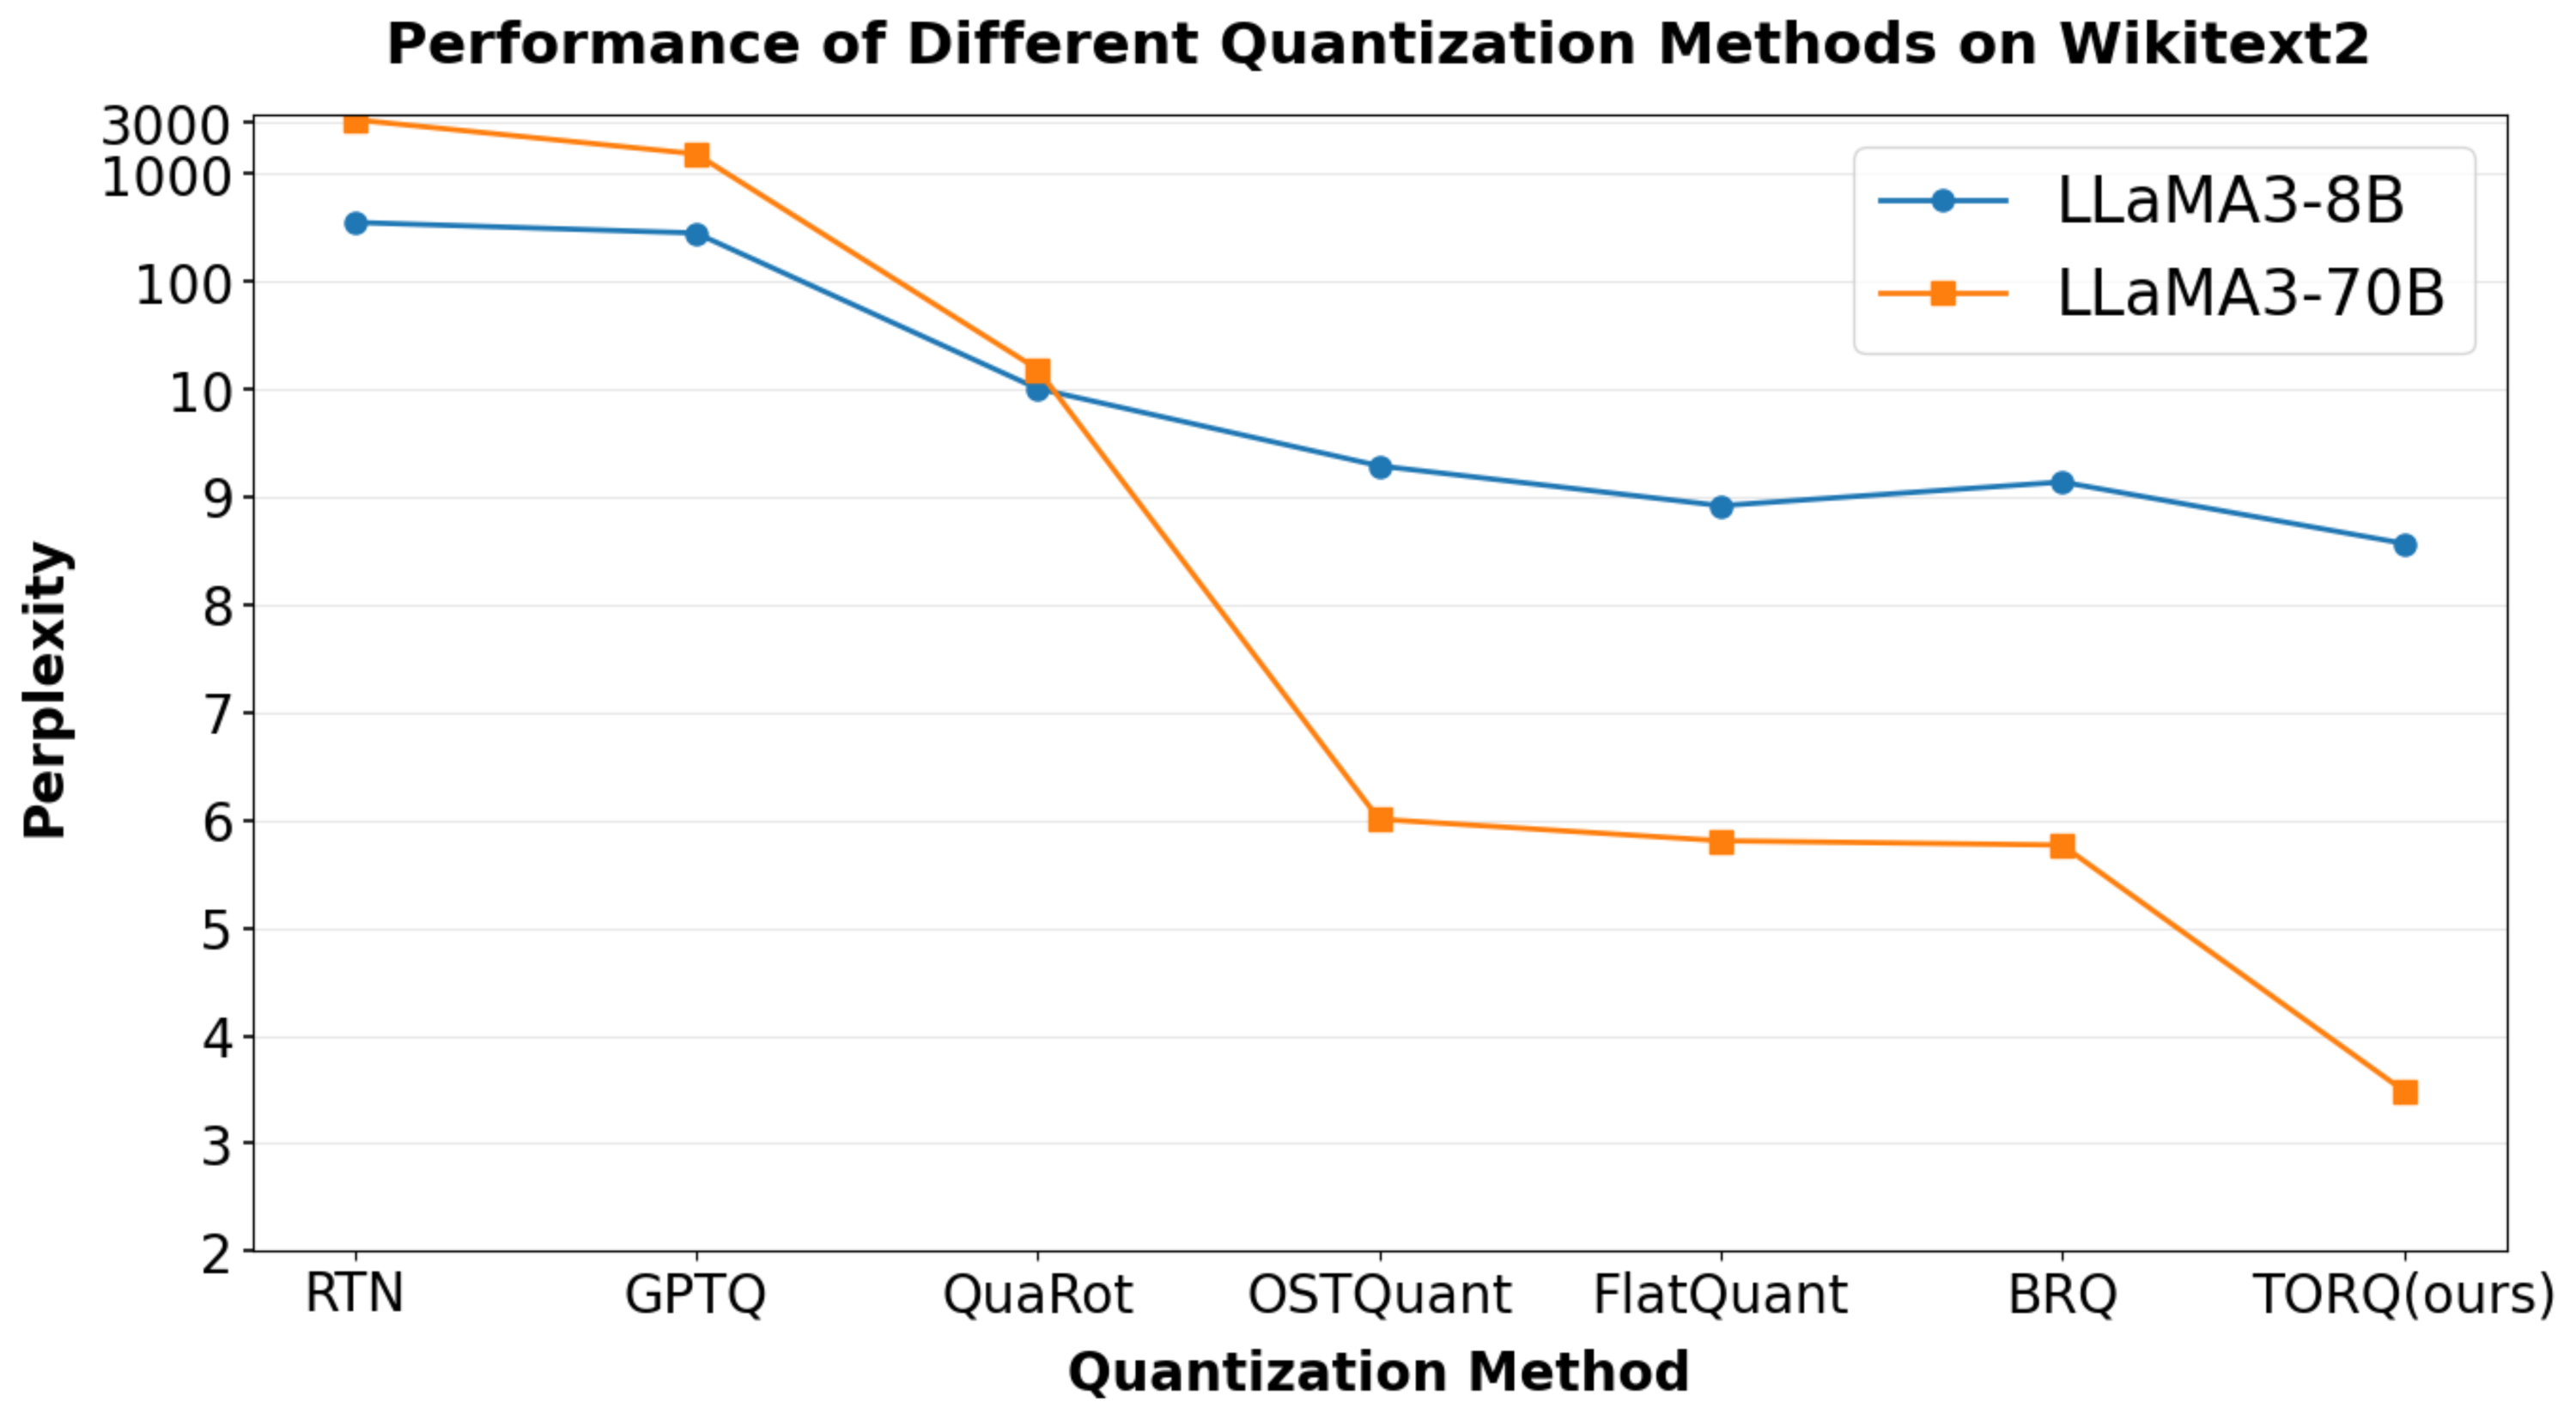
\includegraphics[width=0.45\textwidth]{img/fig_intro_ppl.png}
    \caption{Performance of Different Quantization Methods on LLaMA3-8B and LLaMA3-70B.}
    \label{fig:quantization_performance}
\end{figure}
% \vspace{-4mm}
Despite the theoretical advantages of MXFP4, our empirical analysis reveals that directly applying it to LLM activation quantization encounters severe accuracy bottlenecks. State-of-the-art quantization methods, such as SingleQuant~\cite{singlequant}, DARTQuant~\cite{dartquant}, FlatQuant~\cite{flatquant}, and OSTQuant~\cite{ostquant}, have successfully addressed W4A4 integer quantization through rotation techniques. However, these methods are primarily designed to suppress outliers to fit the uniform grid of integers. This design overlooks the unique Block Floating Point (BFP) topological structure of MXFP4. As a result, simply transferring rotation strategies optimized for integers to MXFP4 often fails to exploit the potential of the floating-point format and may even be counterproductive.

% 【洞察：阻碍精度的两大结构性失衡--motivation】
% 为了解开这一难题，本文深入剖析了 MXFP4 激活量化的误差结构，揭示了导致精度下降的根本原因在于激活分布与 MXFP4 格式之间存在的两大结构性挑战：1.跨块方差极度不均衡 (Inter-block Variance Imbalance)。MXFP4 的量化精度高度依赖于块内共享指数（Scaling Factor）。当激活向量被切分为固定块（如 Block Size=32）时，块方差呈现显著的重尾分布。少数高能量块不仅主导了总均方误差（MSE），更迫使共享指数剧烈抬升，导致同块内 90% 以上的中小幅值元素由于分辨率不足而归零。2.块内码本利用不均衡 (Intra-block Codebook Collapse)。MXFP4 的 e2m1 码本设计假设数据服从理想的对数正态分布。然而，真实激活分布往往高度集中于零点附近，导致绝大多数数值落在最小量化间隔内，而大量表示能力较强的大值码字处于闲置状态（即 Codebook Collapse）。我们的统计显示，如图2所示，约 50% 的码字区间在实际推理中仅被10%数据激活，造成了严重的比特浪费。
\begin{figure*}[ht!] 
    \centering  
    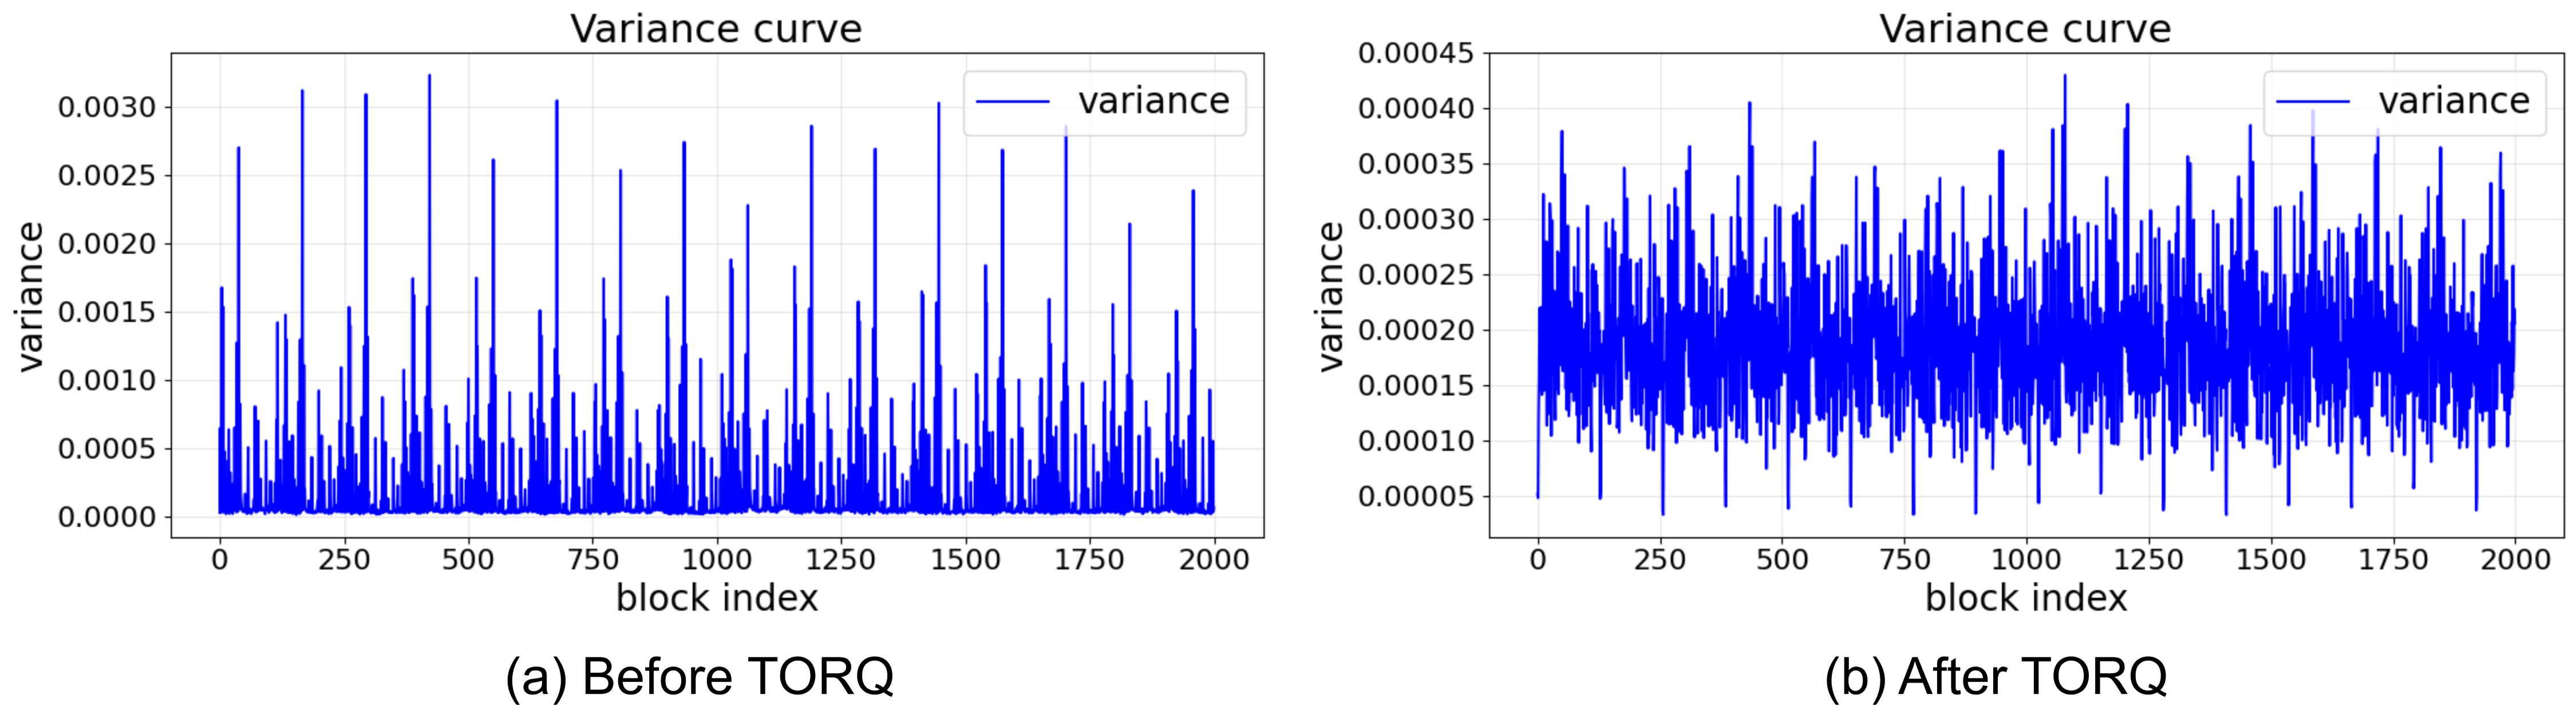
\includegraphics[width=0.95\textwidth]{img/fig-motivation_1.png}
    \caption{MXFP4 Quantization of each micro block's variance distribution: (a) Variance distribution of original data without TORQ, (b) Variance distribution after TORQ processing}
    \label{fig:motivation_1}
\end{figure*}
To address this challenge, this paper conducts an in-depth analysis of the error structure of MXFP4 activation quantization, revealing that the root cause of accuracy degradation lies in two structural conflicts between the activation distribution and the MXFP4 format: (1).Extreme Inter-block Variance Imbalance: The quantization accuracy of MXFP4 relies heavily on the block-wise shared scaling factor. When the activation vector is partitioned into fixed blocks (e.g., Block Size=32), as shown in Figure.\ref{fig:motivation_1}, block variance exhibits a significant heavy-tailed distribution. A minority of high-energy blocks not only dominate the total Mean Squared Error (MSE) but also force the shared exponent to rise sharply, causing over 90\% of small-magnitude elements within the same block to be zeroed out due to insufficient resolution. 
% 【Therefore, our 'Variance Equalization' is not an end in itself, but a mathematically optimal strategy to minimize the maximum required shared exponent across blocks, thereby preserving the precision of non-outlier elements.】
(2).Intra-block Codebook Utilization Imbalance (Codebook Collapse): The e2m1 codebook design of MXFP4 assumes data follows an ideal log-normal distribution. However, real-world activation distributions are often highly concentrated near zero, causing the vast majority of values to fall within the minimum quantization interval, while numerous codewords with strong representation capabilities for large values remain idle (i.e., Codebook Collapse). As shown in Figure.\ref{fig:motivation_2}, our statistics show that approximately 50\% of the codeword range is activated by only 10\% of the data in actual inference, resulting in severe bit waste.
\begin{figure*}[h] 
    \centering  
    
\includegraphics[width=0.95\textwidth]{img/fig-motivation_2.png}
    \caption{Histogram statistics of each codeword quantified by FP4(e2m1):(a) Codeword occupancy of the original data without TORQ, (b) Codeword occupancy after TORQ processing}
    \label{fig:motivation_2}
\end{figure*}

% 【提出我们的方法】
% 基于上述关键洞察，我们提出 TORQ(Two-level Orthogonal Rotation for MXFP4 Quantization) 。这是一种无需重训练的 PTQ 框架，其核心理念是：与其被动调整量化参数以适应病态的激活分布，不如主动旋转激活坐标系，使其分布特性与 MXFP4 的结构特性对齐。TORQ 将优化问题解耦为两个数学上正交的子问题：1.宏观均衡旋转 (Macro-Equilibrium Rotation)：针对跨块方差不均衡，TORQ 基于 Schur-Horn 定理，构造块间正交变换将激活能量在所有块之间均匀“摊平”。我们从理论上证明了，这种方差全均衡配置是最小化全局量化误差的最优解。2.微观对齐旋转(Micro-Alignment Rotation)：针对块内码本利用率低，TORQ 引入最大熵原理，在组内执行正交旋转，重塑局部数据分布，使其在 FP4 空间中均匀“流入”各个码字区间，从而最大化有效信息容量。
Based on these key insights, we propose TORQ (Two-level Orthogonal Rotation for MXFP4 Quantization). This is a retraining-free PTQ framework whose core philosophy is: Instead of passively adjusting quantization parameters to fit ill-conditioned activation distributions, we should actively rotate the activation coordinate system to align its distribution characteristics with the structural properties of MXFP4. 
TORQ decouples the optimization problem into two mathematically orthogonal sub-problems: 
(1).Macro-Equilibrium Rotation: To address inter-block variance imbalance, TORQ constructs an inter-block orthogonal transformation based on the Schur-Horn theorem to uniformly distribute activation energy across all blocks. We theoretically prove that this variance-equalized configuration is the optimal solution for minimizing global quantization error. (2).Micro-Alignment Rotation: To address low intra-block codebook utilization, TORQ introduces the principle of maximum entropy to execute orthogonal rotation within groups. This reshapes the local data distribution to "flow" uniformly into each codeword interval in the FP4 space, thereby maximizing effective information capacity.

% 【我们方法的结果】
% TORQ 仅需少量校准数据即可闭式构造旋转矩阵，且在推理阶段引入的旋转矩阵参数规模极小，几乎不会产生额外计算开销。在 LLaMA、Qwen 等主流大语言模型（LLM）上的实验结果表明，TORQ 的性能显著优于当前的最优方法（SOTA）。如图 3 所示，在 Llama3 系列模型中，该方法的表现始终超越现有的先进量化方案。以 Qwen3-8B 模型为例：在 WikiText 数据集上，其困惑度仅为 10.26，相较浮点模型仅提升 1.26；平均准确率则从 30.73% 大幅提升至 67.75%，较 FlatQuant 方法领先 1.79 个百分点，成功解决了 4-bit 浮点量化场景下的精度下降难题。
% 本文贡献：
%   - 首次系统性地识别并形式化了阻碍 MXFP4 性能的两大结构性挑战——跨块方差不均衡与块内码本利用不均衡 。
%   - 出了首个针对块浮点结构设计的双级旋转框架 TORQ，通过宏观方差均衡与微观码本对齐，实现了量化误差的系统性最小化 。
%   - 为两级旋转建立了坚实的理论基础。证明了在凸误差模型下，方差均衡配置近似最优；同时，论证了在MXFP4几何结构下，码字占用均衡近似于最小化量化误差。
%   - 设计了无需微调的PTQ流程，在多种LLM和多样化的下游任务上验证了方法的有效性、普适性及硬件友好性。

TORQ enables the closed-form construction of rotation matrices using only a minimal volume of calibration data. Furthermore, the rotation matrices incorporated during the inference phase feature an extremely compact parameter footprint, imposing negligible additional computational overhead.Experimental evaluations on mainstream large language models (LLMs), including LLaMA and Qwen, demonstrate that TORQ achieves a significant performance superiority over prevailing state-of-the-art (SOTA) approaches. As illustrated in Figure.\ref{fig:quantization_performance}, this method consistently outperforms existing advanced quantization schemes across the entire Llama3 model series. Taking the Qwen3-8B model as a representative case: on the WikiText dataset, it attains a perplexity score of merely 10.26, representing a marginal increase of 1.26 compared with the full-precision floating-point baseline. Meanwhile, its average accuracy is boosted substantially from 30.73\% to 67.75\%, outperforming the FlatQuant method by a margin of 1.79 percentage points. Collectively, these results confirm that TORQ effectively mitigates the accuracy degradation challenge inherent to 4-bit floating-point quantization scenarios.
Our Contributions:
\begin{itemize}
    \item We systematically identify and formalize, for the first time, the two structural challenges hindering MXFP4 performance: Inter-block Variance Imbalance and Intra-block Codebook Utilization Imbalance.
    \item We propose TORQ, the first dual-level rotation framework explicitly designed for block floating-point structures. By integrating macro-variance equilibrium and micro-codebook alignment, it achieves a systematic minimization of quantization error.
    \item We establish a solid theoretical foundation for two-level rotation. We prove that under a convex error model, the variance equilibrium configuration is approximately optimal; meanwhile, we demonstrate that under the MXFP4 geometric structure, codeword occupancy equilibrium approximates the minimization of quantization error.
    \item We design a fine-tuning-free PTQ pipeline and verify the method's effectiveness, universality, and hardware friendliness across multiple LLMs and diverse downstream tasks.
\end{itemize}
\section{Related Work}
% 传统的LLM量化研究主要围绕INT8/INT4等整数格式展开，其核心在于通过激活感知策略来减小量化精度损失~\cite{illm,mambaquant}。例如，GPTQ通过量化感知微调来调整权重分布，以减轻异常值的影响~\cite{gptq,gptaq}。AWQ提出了一种激活感知的权重量化策略，基于激活统计来保护重要的权重通道~\cite{awq}。SmoothQuant则通过引入可学习的缩放因子，在激活和权重之间重新分配动态范围，从而缓解整数量化中的溢出问题~\cite{smoothquant}。然而，这些方法本质上是在对抗“固定范围”的限制，未能利用浮点格式的动态指数特性。
Traditional research on LLM quantization has primarily revolved around integer formats such as INT8 and INT4, focusing on reducing quantization accuracy loss through activation-aware strategies~\cite{illm,mambaquant}. For instance, GPTQ adjusts weight distributions via quantization-aware updates to mitigate the impact of outliers~\cite{gptq,gptaq}. AWQ proposes an activation-aware weight quantization strategy that protects salient weight channels based on activation statistics~\cite{awq}. SmoothQuant introduces scaling factors to redistribute the dynamic range between activations and weights, thereby alleviating overflow issues inherent to integer quantization~\cite{smoothquant}. However, these methods fundamentally combat the limitations of "fixed ranges" and fail to exploit the dynamic exponent characteristics of floating-point formats.

% 近年来，旋转技术成为量化领域的热点，并成为当前W4A4量化的SOTA方向。QuIP#~\cite{quip_sharp}和QuaRot~\cite{quarot} 引入了 Hadamard 变换以平滑权重和激活的分布；OSTQuant和 FlatQuant虽然在 W4A4 整数量化上取得了 SOTA，但其目标函数旨在压缩数据的动态范围（Clip Ratio Optimization），这与 MXFP4 需要充分利用动态范围的特性并不相符。此外，BRQ~\cite{brq} 虽然尝试了针对 MXFP4 的旋转，但其仅关注块内分布的简单调整，忽略了块间能量失衡这一关键因素。
Recently, rotation techniques have emerged as a focal point in quantization research, representing the current state-of-the-art (SOTA) direction for W4A4 quantization. QuIP\#~\cite{quip_sharp} and QuaRot~\cite{quarot} introduce the Hadamard transform to smooth the distributions of weights and activations. While OSTQuant and FlatQuant have achieved SOTA results in W4A4 integer quantization, their objective functions aim to compress data dynamic range (Clip Ratio Optimization). This objective is incompatible with MXFP4, which requires fully utilizing dynamic range. Furthermore, although BRQ~\cite{brq} attempts rotation for MXFP4, it focuses solely on simple adjustments of intra-block distribution, neglecting the critical factor of inter-block energy imbalance.

% 本文提出的TORQ框架，是首个针对块浮点（Block Floating Point）结构特征设计的双级旋转框架。本文通过“宏观均衡旋转”与“微观对齐旋转”相结合系统性解决了MXFP4激活量化的核心挑战。这一工作填补了针对块浮点结构进行跨块与块内联合分布优化的空白，为低比特浮点格式的激活量化提供了新的优化范式。
The TORQ framework proposed in this paper is the first dual-level rotation framework explicitly designed for the structural characteristics of Block Floating Point (BFP). By combining "Macro-Equilibrium Rotation" and "Micro-Alignment Rotation," we systematically address the core challenges of MXFP4 activation quantization. This work addresses the lack of in joint inter-block and intra-block distribution optimization for block floating-point structures, establishing a new optimization paradigm for low-bit floating-point activation quantization.
\section{Preliminary}
% 符号约定。设某层激活张量$$\mathbf{X}\in\mathbb{R}^{n\times d}$$，其中$$n$$是样Token数，$$d$$为特征维度。我们将$$X$$重排为$$\mathbf{x}\in\mathbb{R}^{B\times K}$$，即$$B$$个块，每个块含$$K$$个元素（通常$$K=32$$）。
% MXFP4量化模型。MXFP4 (e2m1) 采用块级共享缩放因子。对于块向量 $$\mathbf{z}_b \in \mathbb{R}^K$$，量化过程定义为：
% $$\hat{\mathbf{z}}_b = s_b \cdot Q_{\text{mxFP4}}\left( \frac{\mathbf{z}_b}{s_b} \right)$$
% 其中 $$s_b = 2^{\lfloor \log_2(\max(|\mathbf{z}_b|)) \rfloor}$$ 是共享指数（Exponent），$$Q_{\text{mxFP4}}(\cdot)$$ 是将归一化数值映射到 e2m1 离散码本 $$\mathcal{C} = \{\pm 0, \pm 0.5, \pm 1, \pm1.5,\pm2,\pm3,\pm4, \pm 6\}$$ 的最近邻投影算子。
\label{sec:preliminary}

\textbf{Notations.} Let $\mathbf{X} \in \mathbb{R}^{n \times d}$ denote the activation tensor of a specific layer, where $n$ is the number of tokens and $d$ is the feature dimension. We reshape $\mathbf{X}$ into $\mathbf{x} \in \mathbb{R}^{B \times K}$, representing $B$ blocks with $K$ elements each (typically $K=32$).

\textbf{MXFP4 Quantization Model.} The MXFP4 (e2m1) format employs a block-wise shared scaling factor. For a block vector $\mathbf{z}_b \in \mathbb{R}^K$, the quantization process is defined as:
\begin{equation}
\hat{\mathbf{z}}_b = s_b \cdot Q_{\text{mxFP4}}\left( \frac{\mathbf{z}_b}{s_b} \right)
\end{equation}
where $s_b = 2^{\lfloor \log_2 (\max |\mathbf{z}_b|) \rfloor}$ is the shared exponent, and $Q_{\text{mxFP4}}(\cdot)$ is the nearest-neighbor projection operator that maps normalized values to the e2m1 discrete codebook $\mathcal{C} = \{\pm 0, \pm 0.5, \pm 1, \pm 1.5, \pm 2, \pm 3, \pm 4, \pm 6\}$.
\section{Method}
\label{sec:method}
\begin{figure*}[h] 
    \centering  
    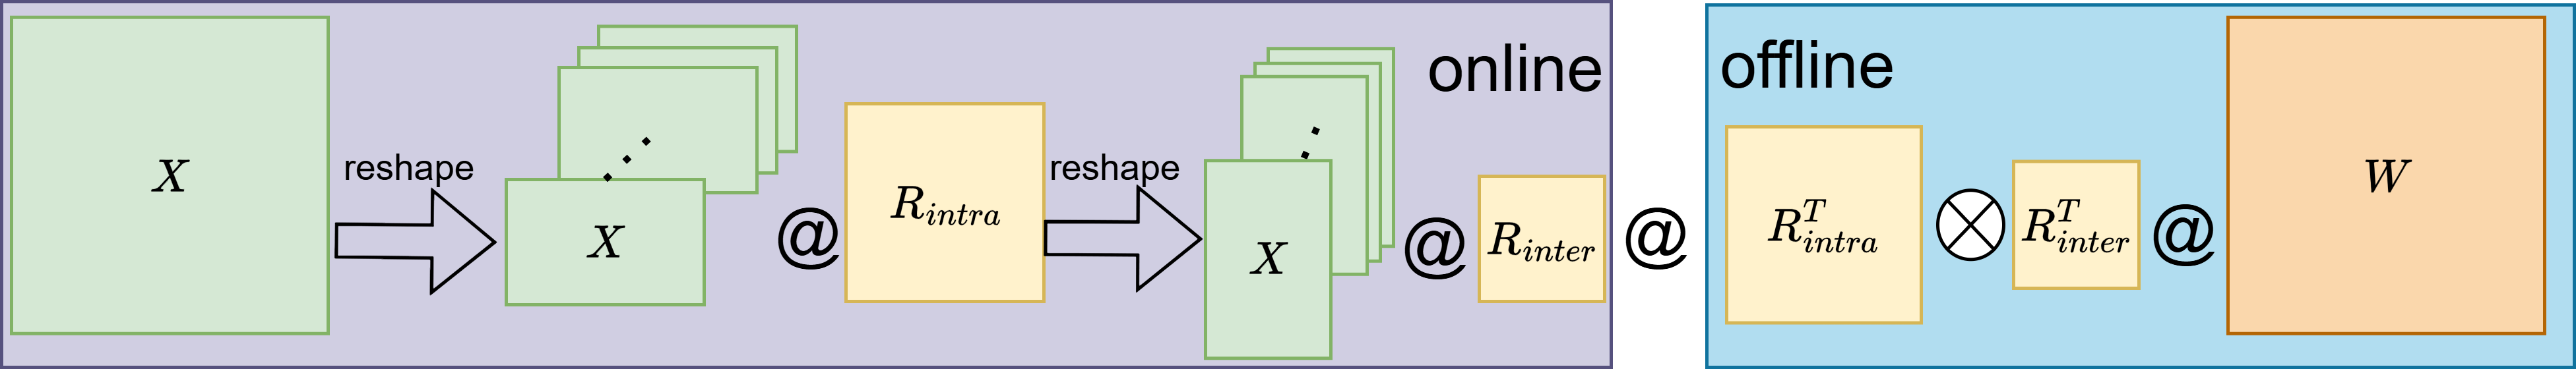
\includegraphics[width=0.95\textwidth]{img/fig-fram.png}
    \caption{TORQ algorithm's complete process framework.}
    \label{fig:fram}
\end{figure*}
% \vspace{-3mm}

Our objective is to find an orthogonal transformation $\mathbf{R} \in \mathcal{O}(d)$ such that the quantization error of the rotated activations $\mathbf{Z} = \mathbf{X}\mathbf{R}$ in the MXFP4 format is minimized:
\begin{equation}
\min_{\mathbf{R} \in \mathcal{O}(d)} \mathbb{E} \left[ \| \mathbf{X}\mathbf{R} - Q_{\text{mxFP4}}(\mathbf{X}\mathbf{R}) \|_F^2 \right]
\end{equation}
Directly optimizing a high-dimensional orthogonal matrix $\mathbf{R}$ is computationally intractable and difficult to converge. To address this, TORQ decomposes $\mathbf{R}$ into two structured sub-transformations: Inter-block rotation $\mathbf{R}_{\text{inter}}$ and Intra-block rotation $\mathbf{R}_{\text{intra}}$, such that $\mathbf{R} = \mathbf{R}_{\text{inter}} \otimes \mathbf{R}_{\text{intra}}$. This decomposition not only reduces optimization complexity but, more importantly, achieves decoupled control over "energy" and "distribution." During the inference phase, the overhead of the inverse transformation can be nearly eliminated by fusing it with the weights of the adjacent linear layer. If the quantized activation $\hat{\mathbf{z}}$ is input to a linear layer $\mathbf{W} \in \mathbb{R}^{d' \times d}$ (where $d = B K$), the fused weight becomes $\mathbf{W}' = \mathbf{W} (\mathbf{R}_{\text{intra}}^\top \otimes \mathbf{R}_{\text{inter}}^\top)$, where $\otimes$ denotes the Kronecker product. Figure.\ref{fig:fram} illustrates the overall framework.

\subsection{Macro-Equilibrium Rotation: Inter-block Rotation based on the Schur-Horn Theorem}

The core objective of inter-block rotation is to achieve global equilibrium of variances across all blocks at the same position via orthogonal transformation, thereby eliminating the dominance of a few high-variance blocks over the total error. The design is based on rigorous convex optimization theory and an efficient engineering construction method.

\subsubsection{Theoretical Foundation: Optimality under Convex Error Models}

For the reshaped activation matrix with structure $B \times K$, assuming the expected mean within blocks is 0, we define the block variance vector $\boldsymbol{\sigma}^2 \in \mathbb{R}^B$, where $\sigma_b^2 = \|\mathbf{z}_b\|_2^2$.

\begin{theorem}[Optimality of Variance Equalization]
\label{thm:optimality}
Assuming the quantization MSE $\phi_b(\sigma^2)$ of block $b$ is a convex function of its input variance $\sigma^2$, the total MSE satisfies:
\begin{equation}
\min_{\mathbf{R}^{(k)} \in \mathcal{O}(B)} \sum_{b=1}^B \phi_b\left([\mathbf{R}^{(k)}\boldsymbol{\Sigma}_k\mathbf{R}^{(k)\top}]_{bb}\right) = \sum_{b=1}^B \phi_b\left(\frac{\mathrm{tr}(\boldsymbol{\Sigma}_k)}{B}\right)
\end{equation}
Equality holds if and only if $\mathrm{diag}(\mathbf{R}^{(k)}\boldsymbol{\Sigma}_k\mathbf{R}^{(k)\top}) = \frac{\mathrm{tr}(\boldsymbol{\Sigma}_k)}{B}\mathbf{1}$ (i.e., all block variances are equal), where $\mathcal{O}(B)$ denotes the group of orthogonal matrices of order $B$, and $\mathbf{1}$ is the all-ones vector.
\end{theorem}

\textit{Proof Sketch.} The Schur-Horn theorem~\cite{schur_horn} states that there exists an orthogonal matrix $\mathbf{R}^{(k)}$ such that the diagonal elements of the transformed covariance matrix can be any vector majorized by the eigenvalues. Under convex functions and constraints, the uniform allocation (constant vector) minimizes the objective function. The complete proof is provided in Appendix A.1.
% The convexity assumption of the error function forms the theoretical basis of Theorem 4.1. In practical engineering, even if the above convexity assumption does not hold, variance smoothing, derived from its outlier suppression mechanism, can still act as an effective "soft limiter" by redistributing the energy of high-variance blocks to low-variance blocks: it reduces the upper limit of the block sharing index ($s_b$), thereby mitigating the quantization noise caused by aggressive scaling.
Beyond the theoretical bounds established by convexity, the practical utility of variance equalization lies in suppressing local maxima. By redistributing energy from high-variance to low-variance blocks, TORQ acts as a dynamic 'soft clipper' that reduces the peak magnitudes determining the shared exponents ($s_b$)2. This effectively lowers the scaling factor ceiling, mitigating the severe resolution loss caused by outliers.

% \begin{lemma}[Convexity of MXFP4 Error Model]
% The block MSE $\phi_b(\sigma^2)$ of MXFP4 block floating-point quantization satisfies convexity. The block MSE of MXFP4 is determined by quantization granularity error, distribution shape factors, and codeword matching factors. Its core term $\exp(2\cdot\mathrm{Var}(\log_2|\mathbf{a}_b|))$ is monotonically increasing and has a non-negative second derivative with respect to block variance $\sigma^2$. Therefore, $\phi_b(\sigma^2)$ is a convex function, satisfying the conditions of Theorem \ref{thm:optimality}. We further demonstrate the convexity of the MXFP4 error model in Appendix A.2.
% \end{lemma}

% \textbf{Key Corollary:} In the context of MXFP4 quantization, a rotation configuration that achieves perfectly balanced inter-block variance is the global optimal solution for minimizing total MSE. This theoretically validates the rationale behind inter-block rotation.

Proposition 4.2 (Empirical Error Behavior). While the strict convexity of the block MSE holds under high-rate quantization assumptions \cite{zamir}, in the coarse 4-bit regime, the error is dominated by the scaling factor $s_b$.

Analysis: The block-wise shared exponent $s
_b$ is determined by the maximum magnitude in the block. Outliers inflate $s_b$, increasing the quantization step size $\sigma=s_b \dot \sigma_{base}$
for all elements. By reducing the variance disparity between blocks (Theorem 4.1), TORQ effectively lowers the expectation of the maximum values, thereby minimizing the average scaling factor and reducing the global quantization noise. Although theoretical convexity is an approximation for discrete FP4, our extensive experiments confirm that variance equalization acts as an effective proxy for MSE minimization.

\subsubsection{Efficient Construction of Orthogonal Matrices: Schur-Horn Driven Givens Rotation}

Based on Theorem \ref{thm:optimality}, we need to construct an orthogonal matrix $\mathbf{R}_{\text{inter}}$ for all position $k$ such that $\mathrm{diag}(\mathbf{R}_{\text{inter}}\boldsymbol{\Sigma}_k\mathbf{R}^\top_{\text{inter}}) = c\mathbf{1}$, where $c=\mathrm{tr}(\boldsymbol{\Sigma}_k)/B$. We design an efficient iterative Givens rotation algorithm (Algorithm \ref{alg:givens}) that ensures convergence within $\mathcal{O}(B^2)$ time.

\begin{algorithm}[tb]
   \caption{Givens Rotation for Variance Equalization}
   \label{alg:givens}
\begin{algorithmic}[1]
   \STATE {\bfseries Input:} Covariance matrix $\boldsymbol{\Sigma} \in \mathbb{R}^{B \times B}$, convergence threshold $\epsilon$
   \STATE {\bfseries Output:} Orthogonal matrix $\mathbf{R} \in \mathcal{O}(B)$ such that $\mathrm{diag}(\mathbf{R}\boldsymbol{\Sigma}\mathbf{R}^\top) \approx c\mathbf{1}$
   \STATE Initialize $\mathbf{R} = \mathbf{I}_B$, calculate target $c = \mathrm{tr}(\boldsymbol{\Sigma})/B$
   \WHILE{$\max_i |\sigma_{ii} - c| > \epsilon$}
       \STATE Select block pair $(i, j)$ with opposite variance deviation signs, i.e., $(\sigma_{ii} - c)(\sigma_{jj} - c) < 0$
       \STATE Calculate rotation angle $\theta = \frac{1}{2}\arctan \frac{2\sigma_{ij}}{\sigma_{ii} - \sigma_{jj}}$
       \STATE Construct Givens rotation matrix $\mathbf{G}_{ij}(\theta)$
       \STATE Update $\boldsymbol{\Sigma} \leftarrow \mathbf{G}^\top \boldsymbol{\Sigma} \mathbf{G}$, $\mathbf{R} \leftarrow \mathbf{R}\mathbf{G}$
   \ENDWHILE
   \STATE {\bfseries return} $\mathbf{R}$
\end{algorithmic}
\end{algorithm}
% \vspace{-6mm}

\subsection{Micro-Alignment Rotation: Intra-block Rotation based on Codebook Alignment}

The goal of intra-block rotation is to reshape the intra-block activation distribution via orthogonal transformation in the normalized MXFP4 codeword space, ensuring that activation values uniformly occupy all available codewords, thereby maximizing the effective utilization of the 4-bit floating-point codebook.

\subsubsection{Computational Graph and Normalized FP4 Space}

Consider the activation matrix $\mathbf{X} \in \mathbb{R}^{B \times K}$ after inter-block rotation. We insert an identity transformation link into the computational graph:
\begin{equation}
\mathbf{X} \xrightarrow[]{\mathbf{S}^{-1}} \mathbf{X}_{\text{norm}} \xrightarrow[]{\mathbf{R}_{\text{intra}}} \mathbf{Z} \xrightarrow[]{Q_{\text{mxFP4}}} \hat{\mathbf{Z}} \xrightarrow[]{\mathbf{R}_{\text{intra}}^\top \mathbf{S}} \hat{\mathbf{X}}
\end{equation}
where $\mathbf{S} = \mathrm{diag}(s_1, \dots, s_B) \in \mathbb{R}^{B \times B}$ is the block-wise scaling matrix with shared scale $s_b$ for each block $b$, and $\mathbf{R}_{\text{intra}} \in \mathbb{R}^{K \times K}$ is the intra-block orthogonal rotation matrix. Under full precision, this link is strictly equivalent to an identity mapping. $\mathbf{S}^{-1}$ normalizes each block to the natural scale of MXFP4 (Normalized FP4 Space), and $\mathbf{R}_{\text{intra}}$ rearranges the statistical distribution of columns within this space.

\subsubsection{Codebook Occupancy Equilibrium Loss}

Let the set of positive codewords for MXFP4 (e2m1) be $\{c_1, \dots, c_J\}$ (where $J=8$), corresponding to decision boundaries $\{d_0=0, d_1, \dots, d_J=+\infty\}$. We define the \textbf{Codebook Occupancy Equilibrium Loss} as:
\begin{equation}
\mathcal{L}_{\text{code}}(\mathbf{S}, \mathbf{R}_{\text{intra}}) = \sum_{j=1}^{J} \left( \hat{p}_j(\mathbf{S}, \mathbf{R}_{\text{intra}}) - \frac{1}{J} \right)^2
\end{equation}
where $\hat{p}_j$ is the empirical codeword occupancy probability. This loss directly quantifies the "imbalance" of MXFP4 codeword usage, aligning precisely with the logarithmic geometric structure of MXFP4.
% 【Discussion on Non-uniformity: We acknowledge that the MXFP4 format is non-uniform, with larger quantization steps in high-value regions (e.g., gap is 2.0 for value 4-6 vs 0.5 for 0-2). Strictly speaking, a uniform histogram (Max Entropy) might push more data into high-error regions compared to an ideal MSE-minimal distribution.
% However, in the context of activation quantization, the dominant failure mode is Codebook Collapse—where most data falls into the zero bin. The gain from "activating" these idle codewords (via Max Entropy) orders of magnitude outweighs the precision loss from the non-uniform grid. TORQ serves as a first-order correction to ensure codebook utilization.】

\subsubsection{Alternating Optimization Framework: S-step and R-step}

We employ an alternating coordinate descent strategy to iteratively optimize $\mathbf{S}$ and $\mathbf{R}_{\text{intra}}$.

\textbf{S-step (Update Block Scaling):} Fix $\mathbf{R}_{\text{intra}}$, and for each block $b$, map its maximum activation value to the maximum MXFP4 codeword $c_{\max}$:
\begin{equation}
s_b \leftarrow \text{clip\_to\_pow2}\left( \frac{\max_i |z_{b,i}|}{c_{\max}} \right)
\end{equation}

\textbf{R-step (Update Intra-block Rotation):} Fix $\mathbf{S}$ and update $\mathbf{R}_{\text{intra}}$ through a series of Givens rotations to monotonically decrease $\mathcal{L}_{\text{code}}$.
\begin{itemize}
    \item \textbf{Column Pair Selection:} Prioritize column pairs with high codebook imbalance and statistical complementarity based on the strategy detailed in Appendix A.5.
    \item \textbf{Angle Search:} For each selected pair $(p, q)$, solve for the optimal Givens rotation angle $\theta^\star$ via one-dimensional search: $\theta^\star = \arg\min_{\theta} \mathcal{L}_{\text{code}}(\mathbf{S}, \mathbf{R}_{\text{intra}} \mathbf{G}_{(p,q)}(\theta))$. Since the loss function is piecewise constant, the optimal solution can be found via finite enumeration (see Appendix A.4).
\end{itemize}

\begin{algorithm}[tb]
   \caption{Intra-block Rotation Construction (Micro Codebook Equilibrium)}
   \label{alg:intra}
\begin{algorithmic}[1]
   \STATE {\bfseries Initialize:} $\mathbf{R}_{\text{intra}}^{(0)} = \mathbf{I}_K$, $\mathbf{S}^{(0)} = \mathbf{I}_B$, $iter=0$
   \WHILE{$iter < MaxIter$ and $\Delta \mathcal{L}_{\text{code}} > \epsilon_{\text{intra}}$}
       \STATE \textbf{S-step:} Update scaling matrix $\mathbf{S}^{(iter+1)}$ using Eq. (5) based on current $\mathbf{R}_{\text{intra}}^{(iter)}$.
       \STATE \textbf{R-step:} Initialize $\mathbf{R}_{\text{current}} = \mathbf{R}_{\text{intra}}^{(iter)}$.
       \STATE Calculate imbalance $h_k$ and select top $K_{\text{top}}$ candidate columns.
       \STATE Select $P$ complementary pairs $\{(p_\ell, q_\ell)\}_{\ell=1}^P$ based on scores $H_{k,l}$.
       \FOR{$\ell=1$ to $P$}
           \STATE Compute optimal angle $\theta_\ell^\star$ for pair $(p_\ell, q_\ell)$ using exact solver.
           \STATE Update $\mathbf{R}_{\text{current}} \leftarrow \mathbf{R}_{\text{current}} \mathbf{G}_{(p_\ell, q_\ell)}(\theta_\ell^\star)$.
       \ENDFOR
       \STATE Update $\mathbf{R}_{\text{intra}}^{(iter+1)} = \mathbf{R}_{\text{current}}$.
       \STATE $iter \leftarrow iter + 1$.
   \ENDWHILE
   \STATE {\bfseries Output:} $\mathbf{R}_{\text{intra}}$, $\mathbf{S}$
\end{algorithmic}
\end{algorithm}
\section{Experiments}
\label{sec:experiments}

\subsection{Experiment Setup}

\textbf{Models and Datasets.} To comprehensively evaluate the universality of our algorithm, we selected the LLaMA-3~\cite{llama3} series and Qwen3~\cite{qwen3} series as foundation models, covering parameter scales from 8B to 70B and including both Dense and Mixture-of-Experts (MoE) architectures. Beyond standard perplexity evaluation on Wikitext2~\cite{wikitext2}, we assessed TORQ on a suite of zero-shot tasks, including ARC-Challenge and ARC-Easy~\cite{arc}, HellaSwag~\cite{hellaswag}, LAMBADA~\cite{lambada}, PIQA~\cite{piqa}, and WinoGrande~\cite{winogrande}. Furthermore, we evaluated performance on more challenging reasoning benchmarks, such as the multi-disciplinary knowledge task MMLU~\cite{mmlu}, the mathematical reasoning benchmark GSM8K~\cite{gsm8k}, and the code generation benchmark HumanEval~\cite{humaneval}.

\textbf{Baseline Methods.} We compared TORQ with current state-of-the-art low-bit quantization methods, including RTN, GPTQ~\cite{gptq}, QuaRot~\cite{quarot}, OSTQuant~\cite{ostquant}, FlatQuant~\cite{flatquant}, and BRQ~\cite{brq}. For fair comparison, all baseline methods were evaluated without GPTQ post-processing, examining solely the quantization performance of the methods themselves.

\textbf{Implementation Details.} All experiments were conducted on NVIDIA RTX 5090 GPUs. We applied MXFP4 quantization to both activations and weights. For calibration, we sampled 128 text segments from the Wikitext2 dataset. As TORQ is an efficient Post-Training Quantization (PTQ) framework, no fine-tuning was performed. For dense models (LLaMA3 and Qwen3), we evaluated MMLU, GSM8K, and HumanEval alongside other zero-shot tasks using the open-source \texttt{lm-evaluation-harness}~\cite{lm_eval}.

\subsection{Main Results}

Table \ref{tab:main_results} presents the main experimental results on the LLaMA3 and Qwen3 model families. \textbf{TORQ significantly outperforms SOTA methods across all tested models and tasks.} 
For example, on LLaMA3-8B, RTN and GPTQ nearly failed in the MXFP4 format (PPL > 280), confirming the challenge of directly applying MXFP4. In contrast, TORQ reduced the WikiText2 perplexity to \textbf{8.57}, surpassing the runner-up methods FlatQuant (8.92) and OSTQuant (9.29). In terms of average accuracy, TORQ achieved \textbf{69.32\%} on LLaMA3-8B, improving by over 37 percentage points compared to the baseline (RTN) and outperforming FlatQuant (68.34\%).

\begin{table*}[h]
\centering
\caption{Main results on LLaMA3 and Qwen3 families. "Wiki2" reports Perplexity ($\downarrow$), and "Avg Acc" reports average accuracy on zero-shot tasks ($\uparrow$).}
\label{tab:main_results}
\resizebox{\textwidth}{!}{
\begin{tabular}{lcccccccccc}
\toprule
 & \multicolumn{2}{c}{\textbf{LLaMA3-8B}} & \multicolumn{2}{c}{\textbf{LLaMA3-70B}} & \multicolumn{2}{c}{\textbf{Qwen3-8B}} & \multicolumn{2}{c}{\textbf{Qwen3-14B}} & \multicolumn{2}{c}{\textbf{Qwen3-32B}} \\
\cmidrule(lr){2-3} \cmidrule(lr){4-5} \cmidrule(lr){6-7} \cmidrule(lr){8-9} \cmidrule(lr){10-11}
\textbf{Method} & Wiki2 & Avg Acc & Wiki2 & Avg Acc & Wiki2 & Avg Acc & Wiki2 & Avg Acc & Wiki2 & Avg Acc \\
\midrule
Baseline (FP16) & 6.14 & 73.18 & 2.87 & 79.95 & 9.00 & 70.43 & 8.64 & 73.81 & 7.61 & 74.82 \\
\midrule
RTN & 354.37 & 32.03 & 3180.43 & 30.92 & 3750.93 & 30.73 & 2219.90 & 35.22 & 274.93 & 38.40 \\
GPTQ & 282.29 & 33.60 & 1532.08 & 34.82 & 1633.38 & 35.54 & 368.24 & 39.91 & 59.31 & 57.62 \\
QuaRot & 10.16 & 62.13 & 15.38 & 62.87 & 23.50 & 55.35 & 20.11 & 60.21 & 18.86 & 61.23 \\
OSTQuant & 9.29 & 65.92 & 6.01 & 73.93 & 19.75 & 54.40 & 16.85 & 64.06 & 14.62 & 67.19 \\
FlatQuant & 8.92 & 68.34 & OOM & OOM & 11.21 & 66.96 & 13.32 & 69.87 & OOM & OOM \\
BRQ & 9.14 & 67.76 & - & - & 13.70 & 64.73 & - & - & - & - \\
\textbf{TORQ (ours)} & \textbf{8.57} & \textbf{69.32} & \textbf{3.49} & \textbf{76.28} & \textbf{10.26} & \textbf{67.75} & \textbf{12.87} & \textbf{70.51} & \textbf{8.43} & \textbf{73.63} \\
\bottomrule
\end{tabular}
}
\end{table*}

\subsection{Ablation Studies}

\textbf{Component Analysis.} To verify the contribution of individual components, we conducted ablation studies on Qwen3-8B (Table \ref{tab:ablation_component}). 
\begin{itemize}
    \item Using only Inter-block Rotation ($\mathbf{R}_{\text{inter}}$) reduced PPL from 3750.93 (RTN) to 24.73, indicating that resolving inter-block variance imbalance is fundamental for recovering model functionality.
    \item Using only Intra-block Rotation ($\mathbf{R}_{\text{intra}}$) lowered PPL to 20.36, demonstrating significant gains from optimizing codebook utilization.
    \item The complete TORQ ($\mathbf{R}_{\text{inter}} + \mathbf{R}_{\text{intra}}$) further reduced PPL to 10.26, boosting GSM8K accuracy to 85.95\%. This proves that macro-variance equilibrium and micro-geometric alignment are orthogonal and complementary.
\end{itemize}

\begin{table*}[h]
\centering
\caption{Ablation study of rotation components on Qwen3-8B.}
\label{tab:ablation_component}
{
\begin{tabular}{cc|cccccc}
\toprule
$\mathbf{R}_{\text{inter}}$ & $\mathbf{R}_{\text{intra}}$ & \textbf{Wiki2} & \textbf{ARC-C} & \textbf{ARC-E} & \textbf{Hella} & \textbf{PIQA} & \textbf{GSM8K} \\
\midrule
\multicolumn{2}{c|}{Baseline (FP16)} & 9.00 & 56.74 & 80.93 & 74.98 & 77.37 & 88.25 \\
\midrule
$\times$ & $\times$ & 3750.93 & 22.94 & 25.07 & 28.73 & 52.11 & 48.93 \\
$\checkmark$ & $\times$ & 24.73 & 40.33 & 60.18 & 55.30 & 61.46 & 65.98 \\
$\times$ & $\checkmark$ & 20.36 & 48.41 & 69.17 & 61.01 & 68.83 & 70.84 \\
$\checkmark$ & $\checkmark$ & \textbf{10.26} & \textbf{53.65} & \textbf{79.36} & \textbf{72.06} & \textbf{74.11} & \textbf{85.95} \\
\bottomrule
\end{tabular}
}
\end{table*}

\textbf{Calibration Dataset Robustness.} We evaluated the sensitivity of TORQ to different calibration datasets on Qwen3-14B (Table \ref{tab:ablation_data}). Results show minimal performance fluctuation (PPL variance < 0.8) across WikiText2, C4, and RedPajama, indicating that TORQ is robust and can capture statistical features from small amounts of generic text.

\begin{table}[h]
\centering
\caption{Robustness across different calibration datasets on Qwen3-14B.}
\label{tab:ablation_data}
\resizebox{0.5\textwidth}{!}{
\begin{tabular}{lcccc}
\toprule
\textbf{Calibration Data} & \textbf{Wiki2} & \textbf{ARC-C} & \textbf{ARC-E} & \textbf{Hella} \\
\midrule
Wiki2 & 12.87 & 55.27 & 81.74 & 76.83 \\
C4 & 13.63 & 56.11 & 81.09 & 78.02 \\
Red\_Pajama & 13.11 & 55.78 & 80.93 & 77.37 \\
\bottomrule
\end{tabular}
}
\end{table}

\textbf{Performance on Hard Tasks.} We assessed "deep intelligence" on MMLU, GSM8K, and HumanEval (Table \ref{tab:hard_tasks}). Traditional methods suffered severe degradation; for instance, GPTQ on Qwen3-8B achieved only 67.37\% on GSM8K and 30.84\% on HumanEval. TORQ recovered GSM8K accuracy to \textbf{86.82\%} (vs. 88.25\% FP16) and HumanEval to \textbf{61.15\%} (vs. 64.63\% FP16), thanks to the micro-alignment rotation preserving fine-grained features critical for reasoning.


\begin{table}[h]
\centering
\caption{Performance on complex reasoning tasks (Qwen3-8B).}
\label{tab:hard_tasks}
\resizebox{0.5\textwidth}{!}{
\begin{tabular}{lcccc}
\toprule
\textbf{Method} & \textbf{MMLU} & \textbf{GSM8K} & \textbf{HumanEval} & \textbf{MathQA} \\
\midrule
Baseline & 74.71 & 88.25 & 64.63 & 49.65 \\
GPTQ & 50.29 & 67.37 & 30.84 & 36.92 \\
QuaRot & 68.88 & 79.30 & 53.37 & 41.12 \\
\textbf{TORQ (ours)} & \textbf{70.82} & \textbf{86.82} & \textbf{61.15} & \textbf{47.94} \\
\bottomrule
\end{tabular}
}
\end{table}
\vspace{-3mm}

\textbf{Generalizability to Other Formats.} We applied TORQ to MXINT4 and NVFP4 formats (Table \ref{tab:formats}). TORQ yielded significant improvements regardless of integer (MXINT4) or floating-point (NVFP4) constraints. Notably, on NVFP4, TORQ improved GSM8K accuracy on Qwen3-8B from 42.67\% (RTN) to 87.08\%, confirming the format-agnostic nature of our geometric optimization.

\begin{table}[!htbp]  % 强制优先当前位置，表格不跑飞
\centering
\renewcommand\arraystretch{1.15}  % 行间距不变，保留你的优化
\caption{Applicability to different microscaling formats (Qwen3-8B).}
\label{tab:formats}  % label在caption后，无hyperref锚点警告
\resizebox{0.5\textwidth}{!}{
\begin{tabular}{c c c cccc}  % ✅ 核心修复：列数精准匹配，无多余&符号
\toprule
\textbf{Format} & \textbf{Method} & \textbf{ARC-C} & \textbf{GSM8K} & \textbf{Hella} & \textbf{PIQA} & \textbf{AVG} \\
\midrule
\multirow{2}{*}{MXFP4} & RTN & 22.94 & 35.87 & 28.73 & 52.11 & 34.92 \\
                       & \textbf{TORQ} & \textbf{53.65} & \textbf{86.82} & \textbf{72.06} & \textbf{74.11} & \textbf{71.66} \\
\midrule
\multirow{2}{*}{MXINT4} & RTN & 23.83 & 37.90 & 30.15 & 50.83 & 35.68 \\
                        & \textbf{TORQ} & \textbf{51.98} & \textbf{85.12} & \textbf{72.72} & \textbf{73.51} & \textbf{70.83} \\
\midrule
\multirow{2}{*}{NVFP4} & RTN & 30.17 & 42.67 & 37.33 & 60.12 & 42.57 \\
                       & \textbf{TORQ} & \textbf{54.38} & \textbf{87.08} & \textbf{73.10} & \textbf{75.83} & \textbf{72.60} \\
\bottomrule
\end{tabular}
}
\end{table}

\textbf{Adaptability to MoE Architectures.} Experiments on Qwen3-30B-A3B (MoE) demonstrated TORQ's effectiveness (Table \ref{tab:moe}). On GSM8K, TORQ achieved 83.83\%, far surpassing GPTQ (37.89\%) and QuaRot (74.18\%), proving its ability to mitigate the heterogeneity of activation distributions across experts.

\begin{table*}[h]
\centering
\caption{Performance on MoE Architecture (Qwen3-30B-A3B).}
\label{tab:moe}
% \resizebox{0.9\textwidth}{!}{
\begin{tabular}{lcccccc}
\toprule
\textbf{Method} & \textbf{ARC-E} & \textbf{ARC-C} & \textbf{Hella} & \textbf{GSM8K} & \textbf{WinG} & \textbf{PIQA} \\
\midrule
Baseline & 79.25 & 56.40 & 79.60 & 85.44 & 70.32 & 80.30 \\
RTN & 24.58 & 26.80 & 25.52 & 22.45 & 52.87 & 51.04 \\
GPTQ & 31.15 & 34.29 & 40.19 & 37.89 & 58.90 & 62.81 \\
QuaRot & 70.45 & 53.19 & 71.14 & 74.18 & 62.51 & 71.11 \\
OSTQuant & 75.84 & 54.03 & 77.23 & 80.28 & 65.80 & 75.09 \\
\textbf{TORQ (ours)} & \textbf{77.10} & \textbf{55.81} & \textbf{78.12} & \textbf{83.83} & \textbf{68.36} & \textbf{77.93} \\
\bottomrule
\end{tabular}
% }
\end{table*}

\subsection{Efficiency Analysis}

\textbf{Speedup and Memory Saving.} As shown in Table \ref{tab:speedup}, on Qwen3-30B-A3B with a 2k context length, TORQ (W4A4) achieves a decoding speed of 220 Toks/s, representing a \textbf{3.5$\times$ speedup} over BF16 (63 Toks/s), while reducing memory usage from 56.9GB to 15.3GB.

\begin{table}[h]
\centering
\caption{Inference speedup and memory footprint on Qwen3-30B-A3B.}
\label{tab:speedup}
\begin{tabular}{lcc}
\toprule
\textbf{Precision} & \textbf{Memory (GB)} & \textbf{Decoder Toks/s} \\
\midrule
BF16 & 56.9 & 63 \\
\textbf{TORQ (W4A4)} & \textbf{15.3} & \textbf{220} \\
\bottomrule
\end{tabular}
\end{table}

\textbf{Quantization Time Comparison.} Unlike training-dependent methods, TORQ's analytical construction is extremely efficient. As detailed in Table \ref{tab:time_cost}, TORQ calibrates Qwen3-32B in just 1920 seconds, which is approximately \textbf{10$\times$ faster than FlatQuant} and \textbf{7$\times$ faster than OSTQuant}, highlighting its practical deployment value.

\begin{table}[h]
\centering
\caption{Comparison of quantization calibration time (seconds).}
\label{tab:time_cost}
\begin{tabular}{lccc}
\toprule
\textbf{Model} & \textbf{OSTQuant} & \textbf{FlatQuant} & \textbf{TORQ} \\
\midrule
Qwen3-8B & 2786s & 3247s & \textbf{427s} \\
Qwen3-14B & 5131s & 6489s & \textbf{893s} \\
Qwen3-32B & 14834s & 18619s & \textbf{1920s} \\
\bottomrule
\end{tabular}
\end{table}

\section{Conclusion}
% 本文针对 MXFP4 作为下一代低精度浮点格式在 LLM 激活量化中面临的核心挑战，提出了 TORQ 两级正交旋转预处理框架。通过系统化分析揭示跨块方差不均衡与块内 FP4 码字使用不均的结构性问题，我们创新性地将量化优化从局部参数调节提升至坐标系设计层面：块间旋转基于 Schur-Horn 定理与凸优化理论，实现跨块方差的全局均衡分配，消除少数高方差块对总误差的支配；块内旋转通过 log₂ 域目标引导与线性域正交变换的协同设计，使激活对数幅值分布逼近均匀，最大化 MXFP4 码字利用率。理论上，我们为两级旋转分别建立了误差下界与优化性质的严格证明；实践中，该方法无需微调、校准成本低且硬件友好，在 LLaMA、Qwen等系列模型及 WikiText、MMLU、GSM8K 等多类任务上，显著缩小了 MXFP4 量化与全精度推理的精度差距，性能超越现有 SOTA 方法 2–5 %。TORQ 不仅为 MXFP4 激活量化提供了首个系统性解决方案，更构建了 “结构感知的正交变换优化” 新范式，为低比特浮点格式在 LLM 高效部署中的应用奠定了关键基础。
This paper addresses the core challenges faced by MXFP4, as a next-generation low-precision floating-point format, in the activation quantization of Large Language Models (LLMs) and proposes the TORQ two-level orthogonal rotation preprocessing framework. Through systematic analysis, it reveals the structural issues of uneven cross-block variance and unequal usage of intra-block FP4 codewords. We innovatively elevate quantization optimization from the level of local parameter adjustment to that of coordinate system design: Inter-block rotation, based on the Schur-Horn theorem and convex optimization theory, achieves the global balanced distribution of cross-block variance, eliminating the dominance of a few high-variance blocks over the total error; Intra-block rotation, through the collaborative design of $log2$ domain target guidance and linear domain orthogonal transformation, makes the distribution of activation logarithmic amplitudes approximate uniformity, maximizing the utilization of MXFP4 codewords. Theoretically, we establish strict proofs for the error lower bounds and optimization properties of the two-level rotations respectively; In practice, this method requires no fine-tuning, has low calibration costs, and is hardware-friendly. On a series of models such as LLaMA and Qwen, as well as various tasks including WikiText, MMLU, and GSM8K, it significantly narrows the precision gap between MXFP4 quantization and full-precision inference, with performance surpassing existing SOTA methods by 2–5\%. TORQ not only provides the first systematic solution for MXFP4 activation quantization but also constructs a new paradigm of "structure-aware orthogonal transformation optimization," laying a crucial foundation for the application of low-bit floating-point formats in the efficient deployment of LLMs.

\section{Limitation}
% 尽管 TORQ 展现出优异的精度与效率权衡，仍存在若干值得进一步探索的局限性：首先，块内旋转当前聚焦于一阶统计（log 幅值期望）的匹配，未能充分利用激活分布的高阶统计信息（如峰度、偏度），在部分激活分布极度非对称或多峰的场景下，可能无法完全释放 FP4 的表达潜力；其次，本文采用固定块大小（如 32）进行实验，而不同模型层、不同任务的激活特性存在显著差异，自适应块大小的动态选择机制及其对量化精度与硬件效率的影响尚未深入研究；最后，虽然我们在 MoE 模型上验证了方法的有效性，但未针对 Expert 间激活分布的异质性设计专属优化策略，对于超大规模 MoE 模型（如 Expert 数量超千级），如何进一步提升跨 Expert 量化一致性仍需探索。这些局限也为未来工作指明了方向，例如结合高阶统计的自适应旋转设计、块大小与模型特性的联合优化等。
Although TORQ demonstrates an excellent trade-off between accuracy and efficiency, there are several limitations that warrant further exploration: First, the current intra-block rotation focuses on matching first-order statistics (the expectation of log magnitudes) and fails to fully utilize the higher-order statistical information of the activation distribution (such as kurtosis and skewness). In scenarios where some activation distributions are extremely asymmetric or multimodal, it may not fully unleash the expressive potential of FP4. Second, this paper uses a fixed block size (e.g., 32) for experiments, while the activation characteristics of different model layers and different tasks vary significantly. The dynamic selection mechanism for adaptive block sizes and its impact on quantization accuracy and hardware efficiency have not been thoroughly studied. Finally, although we verified the effectiveness of the method on MoE models, we did not design specific optimization strategies for the heterogeneity of activation distributions among Experts. For ultra-large-scale MoE models (e.g., with more than a thousand Experts), how to further improve cross-Expert quantization consistency remains to be explored. These limitations also point out directions for future work, such as the design of adaptive rotation combined with higher-order statistics and the joint optimization of block size and model characteristics.


% \nocite{langley00}
\clearpage
\section{Impact Statement}
This paper presents work whose goal is to advance the field of Machine Learning. There are many potential societal consequences of our work, none which we feel must be specifically highlighted here.
\bibliography{example_paper}
\bibliographystyle{icml2026}

\newpage
\appendix
\onecolumn
\input{sec/9.appendix}

\end{document}

% This document was modified from the file originally made available by
% Pat Langley and Andrea Danyluk for ICML-2K. This version was created
% by Iain Murray in 2018, and modified by Alexandre Bouchard in
% 2019 and 2021 and by Csaba Szepesvari, Gang Niu and Sivan Sabato in 2022.
% Modified again in 2023 and 2024 by Sivan Sabato and Jonathan Scarlett.
% Previous contributors include Dan Roy, Lise Getoor and Tobias
% Scheffer, which was slightly modified from the 2010 version by
% Thorsten Joachims & Johannes Fuernkranz, slightly modified from the
% 2009 version by Kiri Wagstaff and Sam Roweis's 2008 version, which is
% slightly modified from Prasad Tadepalli's 2007 version which is a
% lightly changed version of the previous year's version by Andrew
% Moore, which was in turn edited from those of Kristian Kersting and
% Codrina Lauth. Alex Smola contributed to the algorithmic style files.
